\documentclass[a4paper, 14pt]{extarticle}
\usepackage[english,russian]{babel}
\usepackage[T1]{fontenc}
\usepackage[utf8]{inputenc}
\usepackage{fontspec}
\usepackage{indentfirst}
\usepackage{enumitem}
\usepackage{graphicx}
\usepackage[
  left=20mm,
  right=10mm,
  top=20mm,
  bottom=20mm
]{geometry}
\usepackage{parskip}
\usepackage{titlesec}
\usepackage{xurl}
\usepackage{hyperref}
\usepackage{float}
\usepackage[
  figurename=Рисунок,
  labelsep=endash,
  justification=centering
]{caption}
\usepackage[outputdir=build, newfloat]{minted}
\usepackage{chngcntr}

\selectlanguage{russian}

\hypersetup{
  colorlinks=true,
  linkcolor=black,
  filecolor=blue,
  urlcolor=blue,
}

\renewcommand*{\labelitemi}{---}
\setmainfont{Times New Roman}
\setmonofont{JetBrains Mono}[
  SizeFeatures={Size=11},
]

\newenvironment{code}{\captionsetup{type=figure}}{}
\BeforeBeginEnvironment{code}{\bigskip}
\AfterEndEnvironment{code}{\bigskip}

\setminted{
  fontsize=\footnotesize,
}

\setlength{\parskip}{6pt}

\setlength{\parindent}{1.25cm}
\setlist[itemize]{itemsep=0em,topsep=0em,parsep=0em,partopsep=0em,leftmargin=2.0cm,wide}
\setlist[enumerate]{itemsep=0em,topsep=0em,parsep=0em,partopsep=0em,leftmargin=2.0cm,wide}

\renewcommand{\thesection}{\indent\arabic{section}.}
\renewcommand{\thesubsection}{\indent\thesection\arabic{subsection}.}
\renewcommand{\thesubsubsection}{\indent\thesubsection\arabic{subsubsection}.}

\titleformat{\section}{\normalfont\bfseries}{\thesection}{0.5em}{}
\titleformat{\subsection}{\normalfont\bfseries}{\thesubsection}{0.5em}{}
\titleformat{\subsubsection}{\normalfont\bfseries}{\thesubsubsection}{0.5em}{}

\titleformat*{\section}{\normalfont\bfseries}
\titleformat*{\subsection}{\normalfont\bfseries}
\titleformat*{\subsubsection}{\normalfont\bfseries}

\titlespacing{\section}{\parindent}{\parskip}{\parskip}
\titlespacing{\subsection}{\parindent}{\parskip}{\parskip}
\titlespacing{\subsubsection}{\parindent}{\parskip}{\parskip}

\begin{document}

\begin{titlepage}
  \vspace{0pt plus2fill}
  \noindent

  \vspace{0pt plus6fill}
  \begin{center}
    {
    \bfseries
    Министерство науки и высшего образования Российской Федерации
    {
    \scriptsize
    ФЕДЕРАЛЬНОЕ ГОСУДАРСТВЕННОЕ АВТОНОМНОЕ ОБРАЗОВАТЕЛЬНОЕ УЧРЕЖДЕНИЕ ВЫСШЕГО
    ОБРАЗОВАНИЯ
    }
    «Национальный исследовательский университет ИТМО»

    (Университет ИТМО)

    \begin{minipage}[t]{0.42\textwidth}
      \vspace*{0pt}
      \begin{flushright}
        Факультет

        Образовательная программа
      \end{flushright}
    \end{minipage}
    \begin{minipage}[t]{0.57\textwidth}
      \vspace*{0pt}
      \begin{flushright}
        Инфокоммуникационных технологий

        11.03.02 Программирование в инфокоммуникационных системах
      \end{flushright}
    \end{minipage}
    }

    \vspace{0pt plus5fill}

    \LARGE{
      ОТЧЕТ

      по лабораторной работе 5

      по дисциплине \textbf{<<Разработка баз данных>>}
    }
  \end{center}

  \vspace{0pt plus4fill}
  \begin{flushright}
    Выполнил: \textbf{студент группы K33211 Швалов Д. А.}

    Проверил: \textbf{ст. преподаватель Осетрова И.С.}
  \end{flushright}

  \vspace{0pt plus8fill}
  \begin{center}
    Санкт-Петербург

    2024
  \end{center}
\end{titlepage}

\setcounter{page}{2}

\linespread{1.5}
\renewcommand{\baselinestretch}{1.5}

\section*{\large{Лабораторная работа №5 <<Создание представлений>>}}

\section{Цель работы}

Создание представлений.

\section{Задачи, решаемые при выполнении работы}

\begin{enumerate}[leftmargin=*]
  \item Создание представления с помощью SSMS.
  \item Создание представления с помощью представления.
  \item Создание представления с помощью Query Editor.
\end{enumerate}

\section{Объект исследования}

Создание представлений в СУБД \foreignlanguage{english}{Microsoft SQL Server} с
помощью \foreignlanguage{english}{Microsoft SQL Server Management Studio
  (SSMS)}.

\section{Исходные данные}

\begin{itemize}
  \item методические указания к лабораторной работе;
  \item СУБД Microsoft SQL Server;
  \item Microsoft SQL Server Management Studio;
  \item база данных ApressFinancial.
\end{itemize}

\section{Выполнение работы}

\subsection{Первая задача}

\subsubsection{Создания представления с помощью SSMS}

С помощью контекстного меню, показанного на рисунке \ref{fig:task-1-1}, было
открыто окно создания представлений. В окне добавления таблиц, как показано на
рисунке \ref{fig:task-1-2}, была выбрана таблица
<<\foreignlanguage{english}{Shares}>>. После этого в окне создания представления
появилась данная таблица (рисунок \ref{fig:task-1-3}).

Для нового представления были выбраны столбцы
<<\foreignlanguage{english}{Description}>>,
<<\foreignlanguage{english}{StockExchangeTicker}>> и
<<\foreignlanguage{english}{CurrentPrice}>>. Для столбца
<<\foreignlanguage{english}{Description}>> была установлена сортировка по
возрастанию. Для столбца <<\foreignlanguage{english}{CurrentPrice}>> был
установлен псевдоним \foreignlanguage{english}{<<LastPrice>>}, а также
фильтр >0.

Как видно на рисунке \ref{fig:task-1-3}, в сгенерированном запросе появилась
конструкция <<\foreignlanguage{english}{TOP (100) PERCENT}>>. Это произошло из-за
того, что была добавлена сортировка для столбцов представления. Согласно
документации, сортировка в представлениях разрешена только при использовании
конструкции <<\foreignlanguage{english}{TOP}>>.

В окне свойств представления, как показано на рисунке \ref{fig:task-1-4}, была
указана схема <<\foreignlanguage{english}{ShareDetails}>>, а также установлено
поле <<\foreignlanguage{english}{Update Specification}>> в значение
<<\foreignlanguage{english}{No}>>.

После сохранения изменений, новое представление появилось в интерфейсе SSMS
(рисунок \ref{fig:task-1-5}).

\begin{figure}[H]
  \centering
  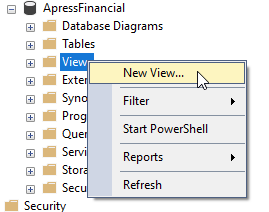
\includegraphics[width=0.4\textwidth]{images/task-1/1.png}
  \caption{Кнопка открытия окна создания представления}
  \label{fig:task-1-1}
\end{figure}

\begin{figure}[H]
  \centering
  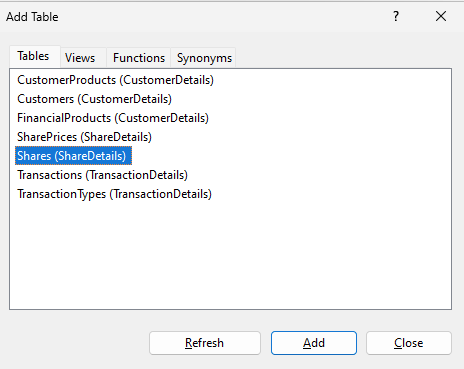
\includegraphics[width=0.7\textwidth]{images/task-1/2.png}
  \caption{Окно добавления таблиц в представление}
  \label{fig:task-1-2}
\end{figure}

\begin{figure}[H]
  \centering
  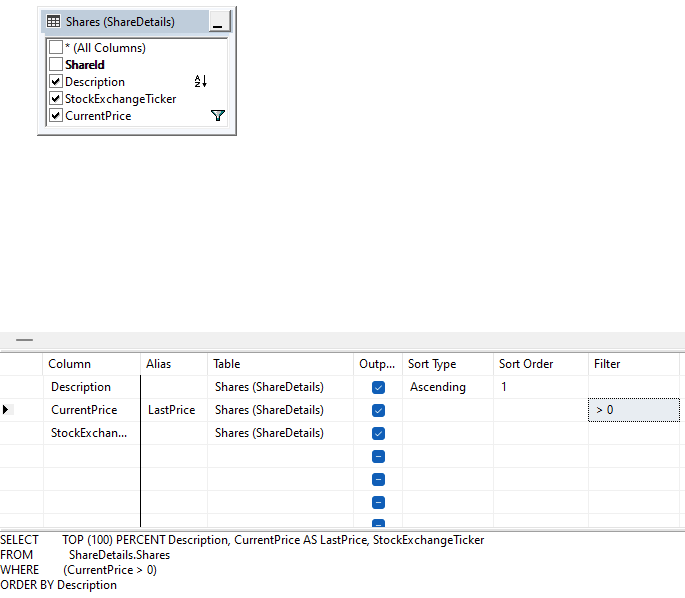
\includegraphics[width=0.8\textwidth]{images/task-1/3.png}
  \caption{Окно создания представления}
  \label{fig:task-1-3}
\end{figure}

\begin{figure}[H]
  \centering
  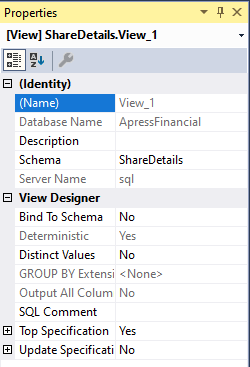
\includegraphics[width=0.35\textwidth]{images/task-1/4.png}
  \caption{Окно свойств представления}
  \label{fig:task-1-4}
\end{figure}

\begin{figure}[H]
  \centering
  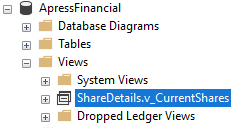
\includegraphics[width=0.5\textwidth]{images/task-1/5.png}
  \caption{Созданное представление}
  \label{fig:task-1-5}
\end{figure}

\subsection{Вторая задача}

\subsubsection{Открытие редактора представлений}

В окне создания представлений были добавлены таблица
<<\foreignlanguage{english}{SharePrices}>> (рисунок \ref{fig:task-2-1}) и
представление <<\foreignlanguage{english}{v\_CurrentShares}>> (рисунок
\ref{fig:task-2-2}). После этого таблица и представление появились в окне
редактирования представления (рисунок \ref{fig:task-2-3}).

\begin{figure}[H]
  \centering
  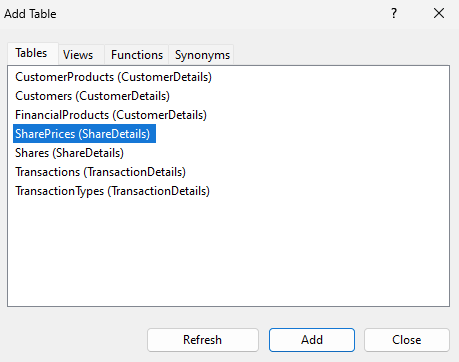
\includegraphics[width=0.7\textwidth]{images/task-2/1.png}
  \caption{
    Добавление таблицы <<\foreignlanguage{english}{SharePrices}>> в
    представление
  }
  \label{fig:task-2-1}
\end{figure}

\begin{figure}[H]
  \centering
  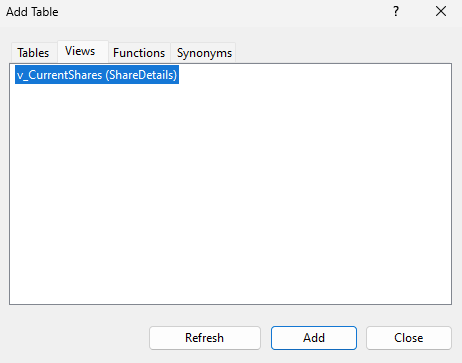
\includegraphics[width=0.7\textwidth]{images/task-2/2.png}
  \caption{
    Добавление представления <<\foreignlanguage{english}{v\_CurrentShares}>> в
    представление
  }
  \label{fig:task-2-2}
\end{figure}

\begin{figure}[H]
  \centering
  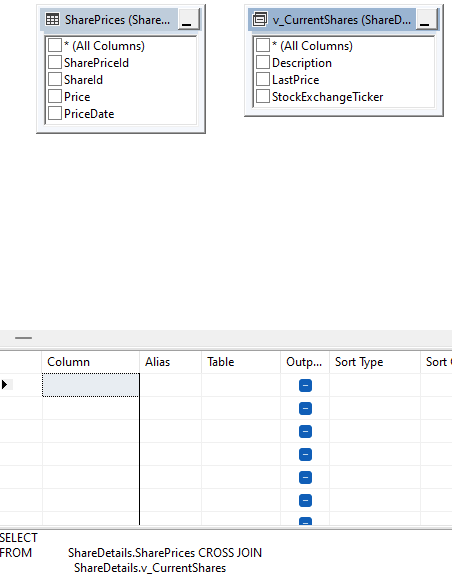
\includegraphics[width=0.5\textwidth]{images/task-2/3.png}
  \caption{Добавленные таблица и представление}
  \label{fig:task-2-3}
\end{figure}

\subsubsection{Создание представления}

С помощью другого редактора представлений, который был открыт с помощью
контекстного меню (рисунок \ref{fig:task-2-4}), в представление
<<\foreignlanguage{english}{v\_CurrentShares}>> был добавлен столбец
<<\foreignlanguage{english}{ShareId}>> (рисунок \ref{fig:task-2-5}). После
этого, как показано на рисунке \ref{fig:task-2-6}, в прежде открытом редакторе у
представления <<\foreignlanguage{english}{v\_CurrentShares}>> появился столбец
<<\foreignlanguage{english}{ShareId}>>.

Как показано на рисунке \ref{fig:task-2-7}, для таблицы и представления была
установлена связь с помощью столбца <<\foreignlanguage{english}{ShareId}>>.
Также для нового представления были выбраны столбцы
<<\foreignlanguage{english}{ShareId}>>, <<\foreignlanguage{english}{Price}>>,
<<\foreignlanguage{english}{PriceDate}>> и
<<\foreignlanguage{english}{Description}>>. Для столбца
<<\foreignlanguage{english}{Description}>> была установлена сортировка по
возрастанию, а для столбца <<\foreignlanguage{english}{Price}>> --- по
убыванию.

После сохранения изменений, новое представление появилось в интерфейсе SSMS
(рисунок \ref{fig:task-2-8}).

\begin{figure}[H]
  \centering
  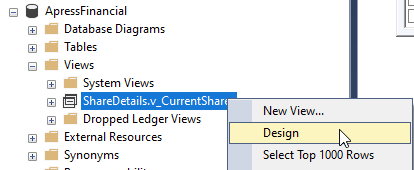
\includegraphics[width=0.7\textwidth]{images/task-2/4.png}
  \caption{Открытие редактора представлений}
  \label{fig:task-2-4}
\end{figure}

\begin{figure}[H]
  \centering
  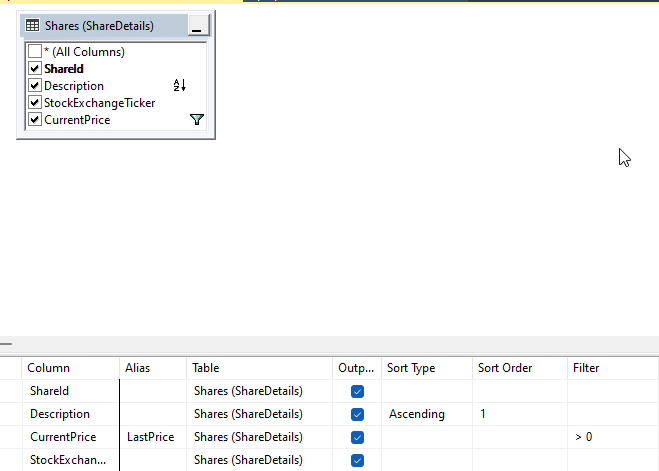
\includegraphics[width=\textwidth]{images/task-2/5.png}
  \caption{Добавление столбца <<\foreignlanguage{english}{ShareId}>>}
  \label{fig:task-2-5}
\end{figure}

\begin{figure}[H]
  \centering
  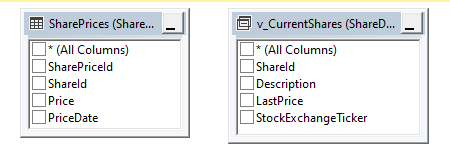
\includegraphics[width=\textwidth]{images/task-2/6.png}
  \caption{Таблица и представление после добавления столбца}
  \label{fig:task-2-6}
\end{figure}

\begin{figure}[H]
  \centering
  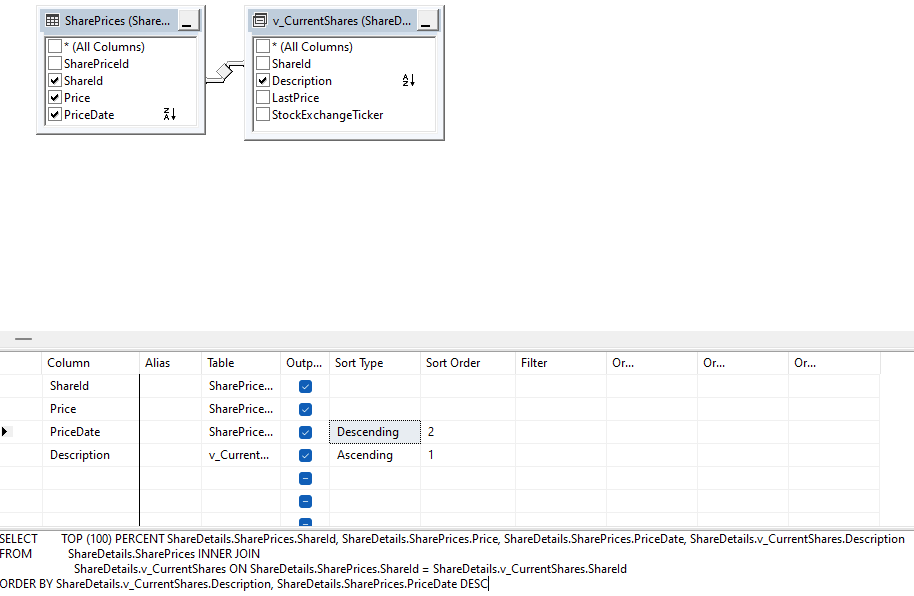
\includegraphics[width=\textwidth]{images/task-2/7.png}
  \caption{Связь между таблицей и представлением}
  \label{fig:task-2-7}
\end{figure}

\begin{figure}[H]
  \centering
  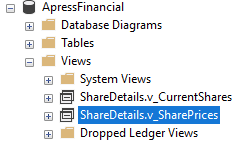
\includegraphics[width=0.5\textwidth]{images/task-2/8.png}
  \caption{Созданное представление}
  \label{fig:task-2-8}
\end{figure}

\subsubsection{Проверка работы представления}

С помощью запроса, показанного на рисунке \ref{fig:task-2-9}, были выведены
строки из представления. Как видно на рисунке \ref{fig:task-2-10}, строки идут
не отсортированы так, как это было указано при создании представления.

\begin{figure}[H]
  \centering
  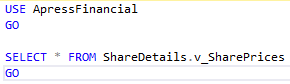
\includegraphics[width=0.7\textwidth]{images/task-2/9.png}
  \caption{Запрос на получение строк}
  \label{fig:task-2-9}
\end{figure}

\begin{figure}[H]
  \centering
  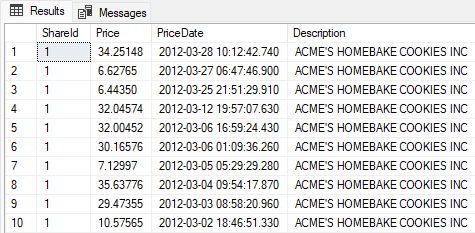
\includegraphics[width=\textwidth]{images/task-2/10.png}
  \caption{Результат выполнения запроса}
  \label{fig:task-2-10}
\end{figure}

\subsubsection{Исправление сортировки}

Для исправления сортировки столбцов был выполнен запрос, показанный на рисунке
\ref{fig:task-2-11}. В нем отсутствует конструкция
<<\foreignlanguage{english}{TOP}>>, поэтому, как показано на рисунке
\ref{fig:task-2-12}, строки теперь выводятся в правильном порядке.

\begin{figure}[H]
  \centering
  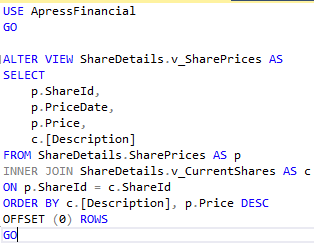
\includegraphics[width=0.7\textwidth]{images/task-2/11.png}
  \caption{Запрос для исправления сортировки}
  \label{fig:task-2-11}
\end{figure}

\begin{figure}[H]
  \centering
  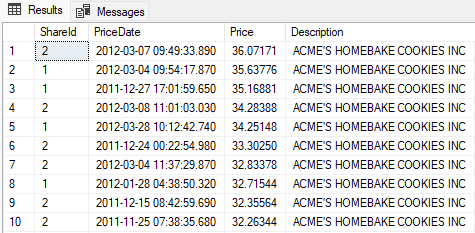
\includegraphics[width=\textwidth]{images/task-2/12.png}
  \caption{Строки из представления}
  \label{fig:task-2-12}
\end{figure}

\subsection{Третья задача}

\subsubsection{Создание представления с помощью Query Editor}

С помощью запроса, показанного на рисунке \ref{fig:task-3-1}, было создано новое
представление <<\foreignlanguage{english}{v\_CustTrans}>>. После выполнения
данного запроса новое представление появилось в интерфейсе SSMS (рисунок
\ref{fig:task-3-2}). На рисунке \ref{fig:task-3-3} показано содержимое
созданного представления.

\begin{figure}[H]
  \centering
  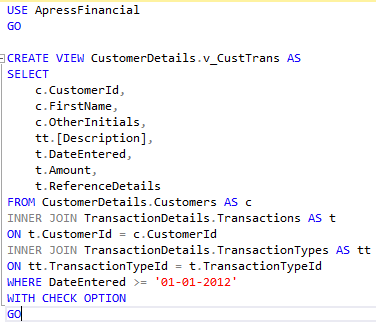
\includegraphics[width=0.7\textwidth]{images/task-3/1.png}
  \caption{Запроса на создание представления}
  \label{fig:task-3-1}
\end{figure}

\begin{figure}[H]
  \centering
  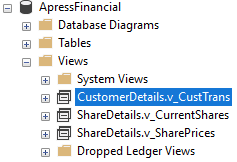
\includegraphics[width=0.5\textwidth]{images/task-3/2.png}
  \caption{Созданное представление}
  \label{fig:task-3-2}
\end{figure}

\begin{figure}[H]
  \centering
  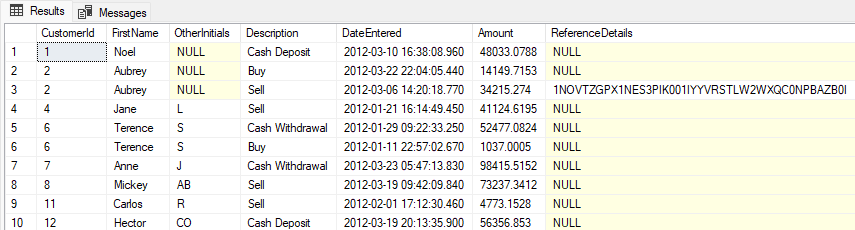
\includegraphics[width=\textwidth]{images/task-3/3.png}
  \caption{Содержимое созданного представления}
  \label{fig:task-3-3}
\end{figure}

\subsubsection{Создание представления с параметром SCHEMABINDING}

На рисунке \ref{fig:task-3-4} показан запрос, в котором сначала удаляется
представление <<\foreignlanguage{english}{v\_CustFinProducts}>>, если оно
существует, а затем создается новое. В данном запросе также используется
параметр <<\foreignlanguage{english}{SCHEMABINDING}>>, который запрещает
изменения схемы таблиц, используемых в представлении. После выполнения запроса,
новое представление появилось в интерфейсе SSMS (рисунок \ref{fig:task-3-5}).
Его содержимое показано на рисунке \ref{fig:task-3-6}.

При попытке изменения таблиц данного представления, например, с помощью запроса,
показанного на рисунке \ref{fig:task-3-7}, возникнет ошибка (рисунок
\ref{fig:task-3-8}).

\begin{figure}[H]
  \centering
  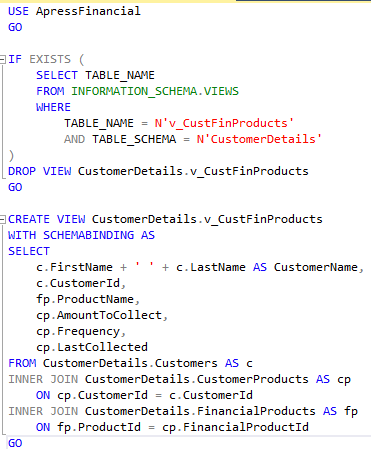
\includegraphics[width=0.5\textwidth]{images/task-3/4.png}
  \caption{Запрос на создание представления}
  \label{fig:task-3-4}
\end{figure}

\begin{figure}[H]
  \centering
  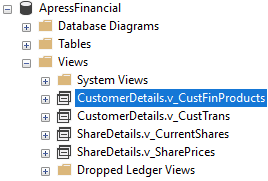
\includegraphics[width=0.5\textwidth]{images/task-3/5.png}
  \caption{Созданное представление}
  \label{fig:task-3-5}
\end{figure}

\begin{figure}[H]
  \centering
  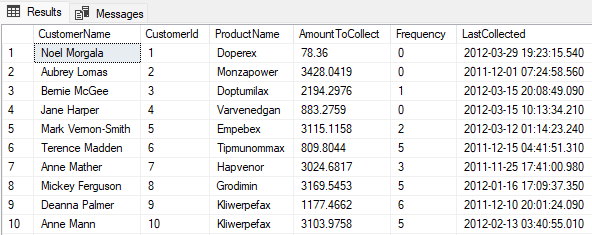
\includegraphics[width=\textwidth]{images/task-3/6.png}
  \caption{Содержимое созданного представления}
  \label{fig:task-3-6}
\end{figure}

\begin{figure}[H]
  \centering
  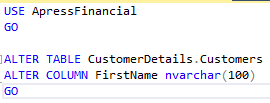
\includegraphics[width=0.6\textwidth]{images/task-3/7.png}
  \caption{Запрос на изменение столбцов таблиц, используемых в представлении}
  \label{fig:task-3-7}
\end{figure}

\begin{figure}[H]
  \centering
  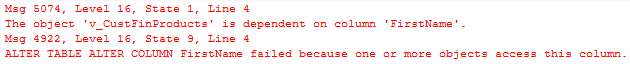
\includegraphics[width=\textwidth]{images/task-3/8.png}
  \caption{Ошибка при изменении столбцов таблиц, используемых в представлении}
  \label{fig:task-3-8}
\end{figure}

\subsubsection{Создание индексированного представления}

С помощью запроса, показанного на рисунке \ref{fig:task-3-9}, был создан
уникальный кластеризованный индекс
<<\foreignlanguage{english}{IX\_CustFinProds}>> для представления
<<\foreignlanguage{english}{v\_CustFindProducts}>>. После выполнения данного
запроса в интерфейсе SSMS появился новый индекс (рисунок \ref{fig:task-3-10}).

\begin{figure}[H]
  \centering
  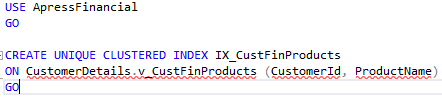
\includegraphics[width=0.7\textwidth]{images/task-3/9.png}
  \caption{Запрос на создание индекса представления}
  \label{fig:task-3-9}
\end{figure}

\begin{figure}[H]
  \centering
  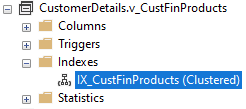
\includegraphics[width=0.5\textwidth]{images/task-3/10.png}
  \caption{Созданный индекс}
  \label{fig:task-3-10}
\end{figure}

\section{Выводы и анализ результатов работы}

В данной лабораторной работе изучены способы создания представлений в SSMS.
Цель, поставленная в начале работы, достигнута, задачи выполнены.

\end{document}
